\section{Methodology}
\label{methodology}

\subsection{Construction of Recurrent Convolutional Neural Network}
\label{RCNN}
RCNN(Recurrent Convolutional Neural Network) has been proved to be very useful for video caption, description and classification \cite{Donahue2015Long}\cite{Aafaq2019Spatio}, however, only a few work apply RCNN to medical image analyze. Recently, Zreik, Majd et al. \cite{Zreik2018A} recently use RCNN for automatic detection and classification of coronary artery plaque, they use CNN extracts features out of $ 25\times25\times25$ voxels cubes, and  use an RNN to process the entire sequence using gated recurrent units (GRUs)\cite{chung2014empirical}. They proved that RCNN's potential for sequence information processing of medical images. 

As mentioned in section~\ref{intro}, CT allows visualization of lung structures, which brings a large amount of redundant information, like muscle,
slices of CT scans can be seen as video frames, so in this study, we use RCNN to capture visual features from CT slices.

Follow the study\cite{Donahue2015Long}, we use LSTM as our RNN cells cause LSTM has been demonstrated to be capable of large-scale learning of sequence data. We test three kinds of classic CNN models: VGG\cite{simonyan2015very}, ResNet\cite{he2016deep} and GoogLeNet with Inception-V3 \cite{szegedy2016rethinking}. 
We wanted to test deeper CNN models like ResNet101, but it will cost a lot of calculation resource, so we give up. Experiments will be discussed in section~\ref{experiments} and section~\ref{discuss}.

We use CNN without fully-connected layers as feature extractor. The input size of CNN is $512 \times 512$, so the outputs of CNN will be very large. We use global average pooling\cite{lin2014network}, as shown in Fig~\ref{gap}, to greatly reduce the number of neurons. It is a replacement of fully-connected layers to enable the summing of spatial information of feature maps. After global average pooling, we insert a fully-connected layer to reduce dimensions to $256$ and fit the requirements of LSTM. Following study in \cite{Donahue2015Long}, the number of LSTM units is set to $256$.

\begin{figure}[htb]
    \centerline{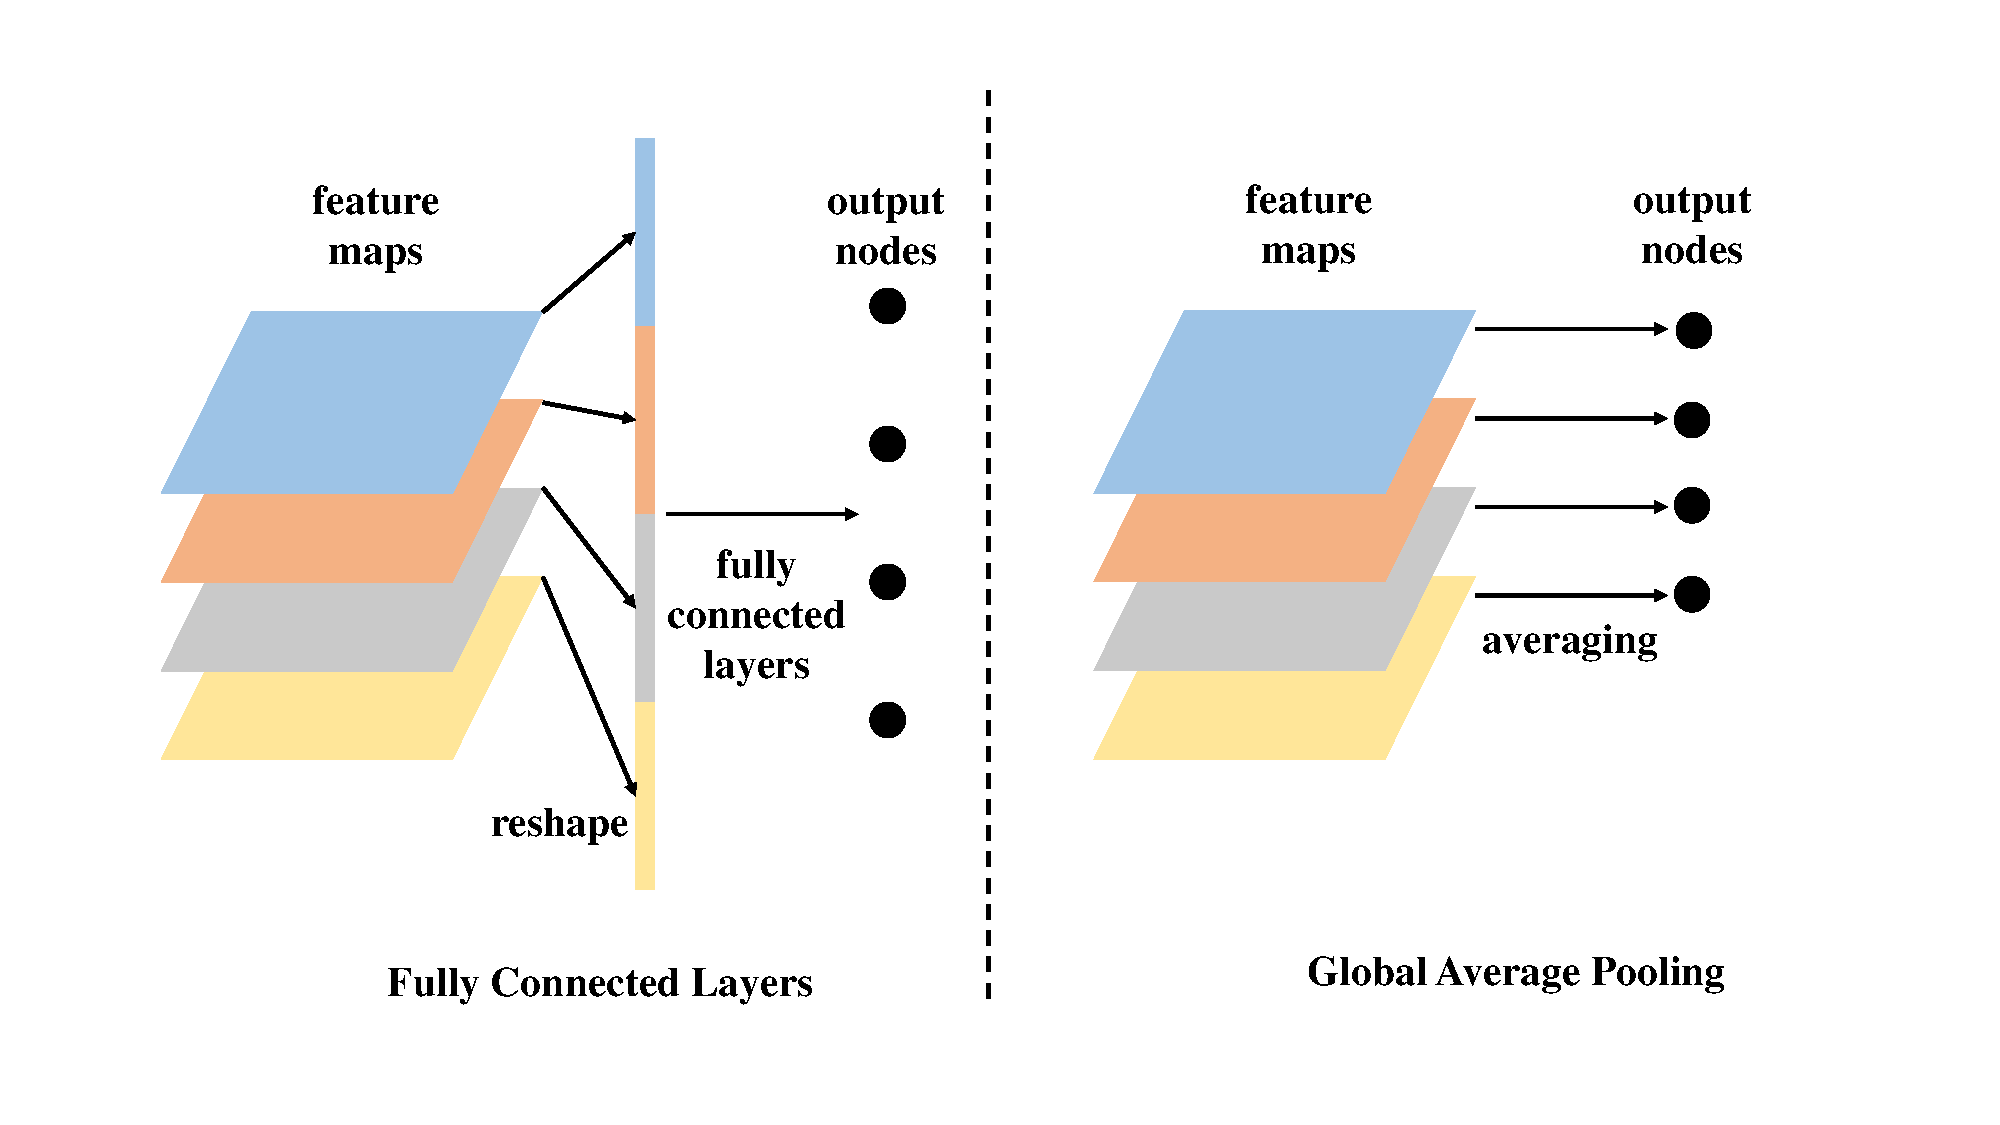
\includegraphics[width=90mm]{gap.pdf}}
    \vspace{-0cm}
    \caption{Difference between Fully Connected Layers and Global Average Pooling}
    \vspace{-0cm}
    \label{gap}
    \end{figure}

For example, if we use ResNet50, the final feature maps will be $16 \times 16 \times 2048$. If we use fully-connected layer, the length of first fully-connected layer will be $1 \times 524288$, which will make model very hard to train. 
If we use global average pooling, outputs from CNN will be reshaped into a tensor with size $1 \times 2048$, then it will be easy to reduce the tensor to $1 \times 256$ using one fully-connected layer. If we have $n$ slices, these slices will be transformed into a matrix with size $n \times 256$, then this matrix will be fed into LSTM by $n$ steps.

In order to get the best RCNN for CT scans, we run experiments to get the best combination between CNN models and LSTM. Architecture of RCNN in this part is shown in Fig~\ref{onestream}. After LSTM layer, we insert two fully-connected layers to give out classification results of RCNN, so that we can observe performances of different RCNNs and choose appropriate architecture. After building RCNN, we will keep architecture above LSTM(including LSTM) and insert into our MDDNet as encoder of visual features.

The experiments show that ResNet50 performs the best in these three models, so our RCNN use ResNet50 as its CNN part, and use one layer of LSTM cells as its RNN part. This conclusion is similar to \cite{Wang2017ChestX}, their experiments showed that ResNet50 outperformed GoogLeNet and VGG16.

\begin{figure*}[t]
    \centerline{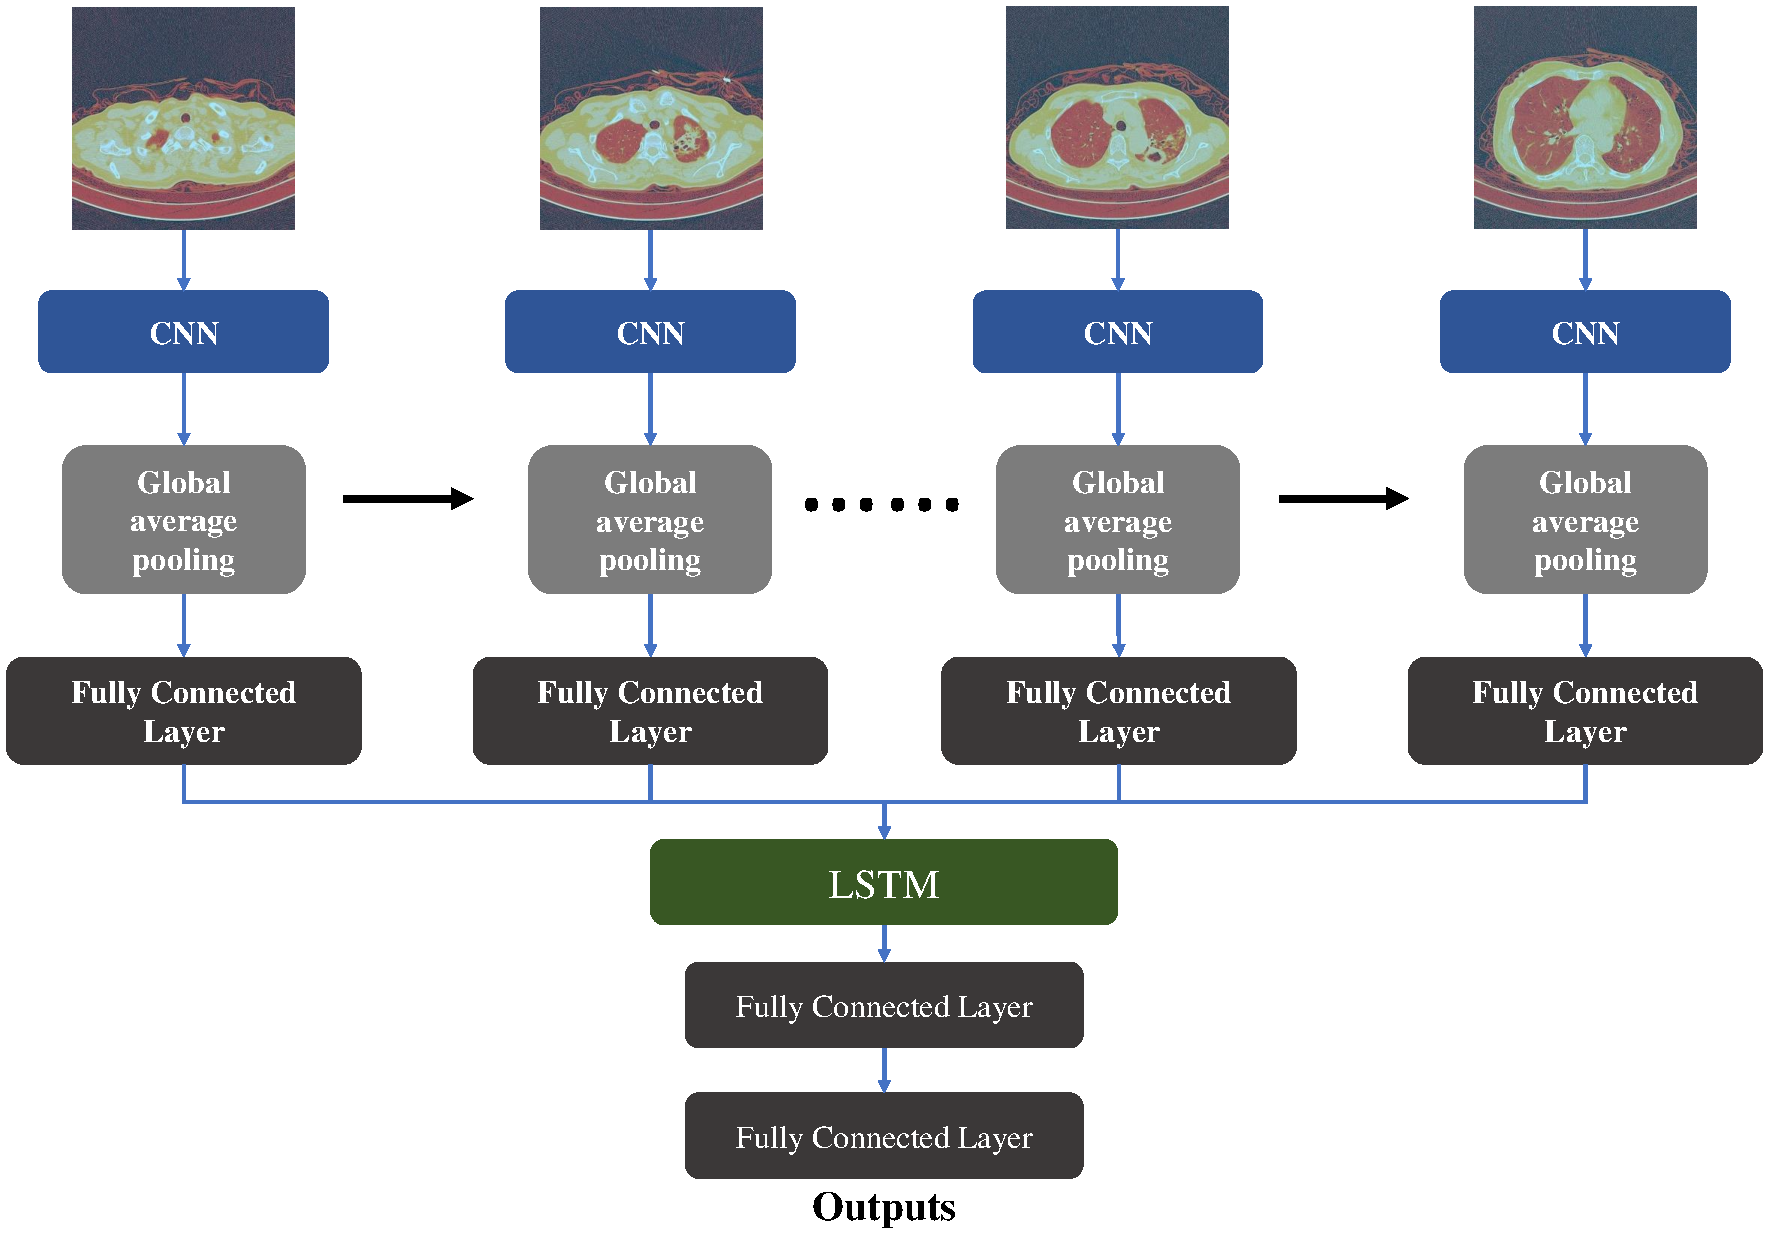
\includegraphics[width=150mm]{onestream.pdf}}
    \vspace{-0cm}
    \caption{Architecture of RCNN}
    \vspace{-0cm}
    \label{onestream}
    \end{figure*}

\subsection{Multimodal Data Fusion and Diagnosis}
\label{MMDDtxt}

The whold RCNN, as mentioned in section~\ref{RCNN}, can be seen as a encoder of CT images, it encodes image feature sequences and gives out the output of the last step as middle state $hv_t$:
\begin{equation}
hv_t = LSTM(Fx_t, hv_{t-1}, z_{t-1})
\label{hvt}
\end{equation}
$Fx_t$ is the $t$-th visual features in CT slices, $hv_{t-1}$ is LSTM hidden state of $t-1$ step, $z_{t-1}$ is LSTM output of $t-1$ step. $t$ is the length of slices, in this study, we set $t$ as 32.

Besides CT image information, we also have clinical information about patients gender, age, and complaints. For gender and age, we use them as additional features and set a tensor with size $1 \times 2$ to hold both values. For patients' complaints, we will use Jieba Chinese word segmentation tool $\footnote[1]{https://github.com/fxsjy/jieba}$ to segment Chinese sentences into word sequences. We set length of Chinese word sequence to 16. Then we transform sequences of words into sequences of vectors using word2vec, which is commonly used in nature language process, since it can capture the relations between words. The width of vectors is set to 50, so does the number of LSTM units. Details of processing steps will be discussed later in section~\ref{experiments}. This LSTM is the second encoder to encode complaint. It is calculated in the same way as Eq.~\ref{hvt}:
\begin{equation}
    hc_{ct} = LSTM(Cx_{ct}, hc_{ct-1}, z_{ct-1})
    \label{hct}
\end{equation}
$Cx_{ct}$ is word embedding matrix of the $ct$-th word in complaint, $hc_{ct-1}$ is LSTM hidden state of $ct-1$ step. $ct$ is the length of complaint, which is 16. 

After getting $hv_t$, $hc_{ct}$, we can calculate the prediction and loss $\Phi_1$ as follows:
\begin{align*}\label{classifyandloss1}
    \Phi_1 &= \sum_i{y_i log(\Delta_i)}, \\
    \Delta &= Softmax(F(hv_t \bigotimes hc_{ct} \bigotimes A \bigotimes G))
\end{align*}
where $y_i$ are vectors for the labels of patients, $\Delta$ is prediction after Softmax, $\bigotimes$ is the concatenation operation, $A$ is patient age, $G$ is patient gender. $F$ is a function to calculate joint distributions of $hv_t$, $hc_{ct}$, $A$ and $G$. In this study, we use two fully-connected layers to fit the function. $\Phi_1$ is cross-entropy that can be used as classification loss \cite{Zreik2018A}.

Since LSTM need to encode 32 visual features, we assume that the gradients propagate to CNN will be very small, so that CNN will not be trained properly. Invoked by study in \cite{szegedy2016rethinking}, we use a auxiliary loss to enhance signal of gradient for CNN.
The auxiliary loss $\Phi_2$ and loss of whole model $Loss$ are defined as follow: 
\begin{align*}
Loss &=  (1 - \omega) \times \Phi_1 +  \omega \times \Phi_2 \\
\Phi_2 &= \sum_i{y_i log(\Delta^c_i)}
\end{align*}
where $\omega$ is a parameter within the interval (0, 1). $\Phi_2$ is classification cross-entropy loss from CNN, $\Delta^c_i$ is Softmax prediction of CNN. $\omega$ can adjust the weight of two losses at different training phases.
We expect that at the beginning of training, CNN get stronger gradient and learn to capture features from CT images more quickly. After parameters of CNN get stable, $\Phi_1$ tends to get small and keep updating parameters of LSTM. We output weights of two losses during training MDDNet, as shown in Table~\ref{weights}, weight for LSTM loss ($1 - \omega$) is 0.6238 at the beginning of training (602 steps), however, ($1 - \omega$) will increase to 0.7234 when training process comes to 36120 steps, it meas weight for CNN is 0.3762 at 602 steps, and it will drop to 0.2766 at the end. Experiments also show that RCNN with auxiliary loss can have a better performance, which will be discussed latter in section~\ref{experiments}.

Finally, MDDNet is built, RCNN for image data and LSTM for clinical information will be trained jointly, the architecture of MDDNet is shown in Fig~\ref{MMDD}. 



\begin{table}[t]
    \vspace{-0cm}
    \caption{Weights of Two Losses at Different Training Step}
    \vspace{-0cm}
    \begin{center}
    \begin{tabular}{|c|c|c|}
    \hline
    \textbf{\textit{Number of Steps}} & \textbf{\textit{$1 - \omega$}} & \textbf{\textit{$\omega$}}\\
    \hline
    602 &0.6238 & 0.3762  \\
    9030 &0.6547 & 0.3453  \\
    18060 &0.7027 & 0.2973  \\
    27090 &0.7185 & 0.2815  \\
    36120 &0.7234 & 0.2766  \\

    \hline
    \end{tabular}
    \vspace{-0cm}
    \label{weights}
    \end{center}
    \vspace{-0cm}
    \end{table}

\subsection{Training Process}
\label{trainingprocess}
There two steps during training process.
The first step is to train difference kinds of RCNN to get the best combination between CNN models and LSTM, the outputs from RCNN($1 \times 256$) will be feed into two fully connected layers to get classification results, as shown in Fig~\ref{onestream}. We compare three kinds of classic CNN models: VGG16, GoogLeNet with Inception-V3, ResNet50. Experiments show that ResNet50 has the best performance. We tried to use deeper network like ResNet101, however using ResNet101 makes the training of model very slow and bring a heavy burden to servers. So we decide to use ResNet50 in RCNN. Moreover, we use CNN models pre-trained on ImageNet \cite{ILSVRC15}. Models without pre-training is almost impossible to train because it won't converge or converge very slow during training. We test difference RCNNs, and experiments show that using pre-trained models can significantly improve the converging speed, as shown in Table~\ref{pretrain}.

The second step is to train MDDNet model. We use RCNN get in the first step as encoder for CT scan visual features, use LSTM as feature encoder for complaints, and combine them with information of age and gender. All these features will be feed into two fully-connected layers and one Softmax layer to get final classification results. Initial learning rate is set to 0.0005 and drops 50\% every 3000 training steps. The dropout rate in fully-connected layers is set to 0.5.

MDDNet will be trained for 4 epoch, and each epoch contains 15 iteration for all training data.

\begin{table}[htb]
    \vspace{-0cm}
    \caption{Comparison between Training from Scratch and Training with Pre-trained Weights}
    \vspace{-0cm}
    \begin{center}
        \begin{tabular}{|c|c|c|c|}
        \hline
        \textbf{\textit{Structure}} & \textbf{\textit{Pre-trained}} & \textbf{\textit{Data}}& \textbf{\textit{Accuracy}}  \\
        \hline
        RCNN(ResNet) &No & Lung Window Image & 0.545\\
        RCNN(GoogLeNet) & No & Lung Window Image & 0.545\\
        RCNN(ResNet) & Yes & Lung Window Image & 0.925\\
        RCNN(GoogLeNet) & Yes & Lung Window Image & 0.865\\
        
        \hline
        \end{tabular}
    \vspace{-0cm}
    \label{pretrain}
    \end{center}
    \vspace{-0cm}
    \end{table}
